\chapter{Cartan's test}\label{chapter:test}
\chapterSummary{We explain how involutivity can be seen as having the generic integral line lie in an integral plane and so on.}%
\section{Generic points and generic submanifolds}
When we say that the \emph{generic}\define{generic} point of some manifold has some property, we mean that those points which fail to have that property lie in a closed, nowhere dense set.
The \emph{generic} submanifold has some property if the property holds for all submanifolds whose tangent spaces avoid some closed, nowhere dense subset of the Grassmann bundle.
The definition of \emph{generic} in analysis is usually more sophisticated; we could use a more sophisticated definition without changing any of our proofs or results, but we won't need to.

\section{Cartan's strategy}
Draw a point, an integral curve through that point, an integral surface through that curve, and so on up to some required dimension.
We fail unless the integral curve is \emph{extendable}, i.e. lies inside an integral surface, and so on.
Integral curves are not always extendable.
Don't try to draw all integral curves, surfaces, and so on, but only the generic ones: ask whether the generic integral curve is extendable, and the generic integral surface, and so on.

\section{Cartan's test}
An integral line is \emph{extendable} if it lies in an integral plane, and so on.
We can imagine that extendability of generic integral manifolds is related to extendability of generic integral elements.
\prob{test:ext}{Prove that any integral element is extendable just when its codimension, in the space of integral elements, exceeds the rank of its polar equations.}

A \(0\)-dimensional integral element is \emph{regular}\define{regular!integral element}\define{integral!element!regular} if its polar equations have locally maximal rank.
Locally maximal rank is the same as locally constant rank, as linearly independent polar equations remain linearly independent nearby.

An integral element is \emph{ordinary}\define{ordinary!integral element}\define{integral!element!ordinary} if it contains a regular hyperplane, and \emph{regular} if in addition its polar equations have locally maximal rank.
Regularity and ordinarity are difficult to test directly, so we will prove:
\begin{theorem}[Cartan's test]\label{theorem:test}\define{test!Cartan's}\define{Cartan!test}
An integral element is involutive if and only if it is ordinary.
\end{theorem}
\begin{corollary}
In each component of the space of integral elements, either none are involutive or the generic one is involutive.
\end{corollary}
Ordinarity occurs precisely when the generic integral line sits in an integral plane, and so on:
\prob{test:generic}{Prove that an integral plane \(E_2\) is ordinary just when, for any integral line \(E_1\subset E_2\), every integral line close enough to \(E_1\) sits in an integral plane.}
\section{Differentiating on the Grassmann bundle}
Each differential form \(\vartheta\) yields an equation \(0=\vartheta\), satisfied by the integral elements of the exterior differential system it generates.
At any given point \(m_0 \in M\), integral elements are points of the Grassmannian \(\Gr{p}{T_{m_0} M}\).\prob{eds:polar.diff}{Identify the polar equations at an integral element with the differentials of those equations on the Grassmannian.}
\begin{answer}{eds:polar.diff}
Take a \(\vartheta\)-integral element 
\[
E_0=\spn{e_1,e_2,\dots,e_p}.
\]
Move it:
\[
E_t=\spn{e_1+tw_1+O(t)^2,\dots,e_p+tw_p+O(t)^2}.
\]
Every motion through \(p\)-dimensional subspaces has this form locally.
Expand:
\[
\left.\vartheta\right|_{E_t}=t\sum_i \vartheta(e_1,\dots,e_{i-1},w_i,e_{i+1},\dots,e_p)+O(t)^2.
\]
The differentials, i.e. linear terms, are sums of polar equations.
Set all but one \(w_i\) to zero: every polar equation is a differential.
In coordinates, \(E_0=(du=0)\), \(E_t=(du=q(t) \, dx)\), let \(w_i(t)\defeq q^a_i(t)\p{u^a}\).
\end{answer}
\begin{corollary}\label{corollary:same.int.elts}
Take an involutive integral element \(E\) of any exterior differential system \(\II\).
Take a subsystem \(\II'\subseteq\II\) and a flag in \(E\).
If the \(\II'\)-characters of that flag are the \(\II\)-characters of \(E\), then \(\II\) and \(\II'\) have the same integral elements near \(E\), and so the same integral manifolds with tangent spaces near \(E\).
\end{corollary}
\begin{proof}
The \(\II'\)-integral elements lie in a submanifold of the Grassmann bundle, with codimension equal to the number of linearly independent polar equations, by problem~\vref{problem:eds:polar.diff}.
This submanifold has the same dimension as the set of \(\II\)-integral elements, which it contains.
\end{proof}

\section{Extending integral elements}
\begin{lemma}\label{lemma:point.int.elements}
Every ordinary integral element is involutive.
\end{lemma}
\begin{proof}
Impose \(p-1\) generic linear constraints; they cut down our given ordinary integral element \(E\) to an integral line.
They also cut down nearby integral elements to nearby integral lines.
On the other hand, a line satisfying those generic constraints is integral just when it satisfies \(s_0\) linearly independent polar equations.
Pick another \(p-1\) generic linear constraints.
A line satisfying these will sum to our integral line to span an integral plane, just when it satisfies the \(s_0+s_1\) linearly independent polar equations of our integral line.
By induction, the general \(p\)-dimensional integral element near \(E\) is cut out by solving \(ps_0+(p-1)s_1+\dots+s_{p-1}\) equations.
Solutions form an analytic manifold by problem~\vref{problem:v.b.rank}, of dimension \(\dim M+s_1+2s_2+\dots+ps_p\).
\end{proof}
\prob{test:test.thm}{Prove theorem \vref{theorem:test}.}
\begin{answer}{test:test.thm}
If an integral is not ordinary, we can find integral elements nearby with characters ``borrowed'' downward, so larger \(s_0\), or the same \(s_0\) but larger \(s_1\), or some such.
As \(p+s_0+\dots+s_p=\dim M\), borrowing raises one character and lowers some later character, decreasing the dimension 
\[
\dim M + s_1 + 2s_2 + \dots + ps_p,
\]
of the submanifold containing all nearby integral elements.
\end{answer}
\begin{problem}{eds:lower.dim}
Prove that the generic linear subspace \(E_k \subset E_p\) of dimension \(k\) of an involutive integral element is involutive with the same characters \(s_1,s_2,\dots,s_k\) as \(E_p\), up to dimension \(k\).
\end{problem}
\begin{answer}{eds:lower.dim}
Generic linear subspaces are regular, so ordinary, so involutive.
The polar equations along a generic integral element are the same.
\end{answer}
\begin{problem}{test:characterize.int.elts}
Take a subset \(\mathscr{E}\) of a Grassmann bundle of a manifold.
Let \(\mathscr{E}^\perp\) be the set of all differential forms vanishing on all elements of \(\mathscr{E}\).
Use the Cartan--K\"ahler to prove that \(\mathscr{E}\) is an open subset of the set of involutive integral elements of an exterior differential system if and only if \(\mathscr{E}^{\perp}\) is the unique maximal such system.
\end{problem}
\begin{answer}{test:characterize.int.elts}
Clearly \(\mathscr{E}^{\perp}\) is an ideal of differential forms, and homogeneous (i.e. the direct sum of its intersections with forms each degree).
But \(\mathscr{E}^{\perp}\) might not be \(d\)-closed.
Take its \(d\)-closure \(\mathscr{E}^{\vee}\); it has the same integral manifolds as \(\mathscr{E}^{\perp}\).
Suppose that there is an exterior differential system \(\II\) with \(\mathscr{E}\) among its integral elements: 
\[
\II\subset\mathscr{E}^{\perp}\subset\mathscr{E}^{\vee}.
\]
Every \(\II\)-integral manifold has tangent spaces from \(\mathscr{E}\), so an \(\mathscr{E}^{\perp}\)-integral manifold, so an \(\mathscr{E}^{\vee}\)-integral manifold.
So \(\II,\mathscr{E}^{\perp},\mathscr{E}^{\vee}\) share the same integral manifolds.

Suppose now that \(\mathscr{E}\) is an open subset in the set of involutive maximal dimensional \(\II\)-integral elements.
Every element of \(\mathscr{E}\) arises as the tangent space of an \(\II\)-integral manifold, by the Cartan--K\"ahler theorem, so as the tangent space of a \(\mathscr{E}^{\vee}\)-integral manifold.
So \(\mathscr{E}\) lies among the \(\mathscr{E}^{\vee}\)-integral elements, which lie among the \(\II\)-integral elements.
The differential of any form vanishing on \(\mathscr{E}\) lies in \(\mathscr{E}^{\vee}\), so also vanishes on \(\mathscr{E}\).
So \(\mathscr{E}^{\perp}=\mathscr{E}^{\vee}\).

Consider an \(\mathscr{E}^{\vee}\)-integral element \(E\).
Being an \(\II\)-integral element, if \(E\) lies close enough to a linear subspace \(E'\) of some element of \(\mathscr{E}\), then \(E\) lies in a maximal dimensional involutive \(\II\)-integral element, so an element of \(\mathscr{E}\), so in a maximal dimensional \(\mathscr{E}^{\vee}\)-integral element.
So \(\mathscr{E}^{\vee}\) is involutive near \(\mathscr{E}\).
But \(\mathscr{E}^{\vee}\)-integral elements near elements of \(\mathscr{E}\) are \(\II\)-integral elements, so elements of \(\mathscr{E}\).
\end{answer}

\section{View from a tableau}
\begin{problem}{test:local.tableaux}
Prove that, for any involutive integral element \(E\subset T_{m_0} M\) of an exterior differential system \(\II\),  there is a tableau defined near \(m_0\), with characters equal to those of \(\II\), generating an exterior differential system with the same characters and integral elements as \(\II\) near \(E\).
\end{problem}
\begin{answer}{test:local.tableaux}
Pick a tableau at \(m_0\) which is generic in the usual sense:  having maximal \(s_1\) among all tableaux for the same system, and maximal \(s_2\) subject to that \(s_1\), and so on.
Let \(\II'\subseteq\II\) be the exterior differential system generated by  the \(\theta^a\) and the rows of the tableau.
It is possible that various forms in \(\II\) vanish at \(m_0\), and near \(m_0\) lie outside \(\II'\).
Note that the characters of \(\II'\) at any \(\II\)-integral element are no larger than those of \(\II\) since \(\II'\subseteq\II\).

Suppose now that \(\II\) is involutive.
The characters of \(\II\) are locally constant by problem~\vref{problem:eds:lower.dim}.
The characters of \(\II'\) are at least as large as those of the tableau, which match those of \(\II\) at \(m_0\).
So \(\II'\) and \(\II\) have the same characters, and both are involutive on all of their integral elements, with the same dimensions of spaces of integral elements.
Hence they have the same integral elements where the tableau maintains those same characters.
\end{answer}
\begin{problem}{test:absorb}
Prove in addition that locally (not just at a point) some change of coframing absorbs torsion.
\end{problem}
\begin{answer}{test:absorb}
``Generic'' is just a condition on linear independence of \(\pi\) \(1\)-forms, so holds locally.
Torsion is absorbable at a point just when there is a torsion free integral element coframed by \(\omega^1,\dots,\omega^p\).
Absorbing torsion is solving a system of linear equations of constant rank; apply problem~\vref{problem:v.b.rank}
\end{answer}
Put all polars \(\pi^{\alpha}\) of grade \(i\) into the entries of a column vector \(\pi^i\), with \(s_i\) rows.
Write the equations for integral elements by plugging \(\pi^i=p^i_j\omega^j\) into the tableau.
The \emph{grade}\define{grade} of \(p^i_j\) is \(i-j\).

For the moment, suppose there is no nonlinearity.
Plug into the tableau to get linear equations solving for all coefficients \(p^i_j\) for \(i<j\) in terms of various coefficients \(p^{\beta}_i\), with a smaller subscript.
Inductively, we solve for all negative grade coefficients in terms of semipositive grade coefficients (where \emph{semipositive}\define{semipositive} means \emph{not negative}). 
(There may be other equations as well, from entries that are not polars; ignore these.)
We solve for \(p^1_i\), for \(i=2,3,\dots,p\), hence \((p-1)s_1\) equations.
Similarly for the other grades, a total of
\[
(p-1)s_1+(p-2)s_2+\dots+s_{p-1}
\]
equations at least, on \(p(s_1+s_2+\dots+s_p)\) variables.
Each integral element at this point is determined by the values of its semipositive coefficients.
The number of semipositive coefficients is the difference between number of variables and number of equations:
\[
s_1+2s_2+\dots+ps_p.
\]

We assumed no nonlinearity.
Each nonlinearity term puts a quadratic or higher order expression into each of these equations.
By the implicit function theorem, near an integral element, say arranged to be at the origin, higher order terms do not alter the possibility to solve the equations locally analytically.

This tableau is only computed at one point.
Extend the \(1\)-forms in which it is expressed to be defined nearby as well.
Careful: there might be differential forms in \(\II\) which vanish at the point where we computed the tableau; we are ignoring them.
So when we extend the forms of the tableau to nearby points, we obtain a tableau for some subsystem of \(\II\), but maybe not all of \(\II\).

The space of integral elements thus locally lies in a submanifold of the Grassmann bundle of dimension
\[
\dim M + s_1+2s_2+\dots+ps_p,
\]
parameterized by choices of point of \(M\) and semipositive grade coefficients.
Near a given integral element, the space of integral elements is a submanifold of that dimension just when the tableau is involutive at that integral element.
Involutivity holds just all other equations arising on integral elements are consequences of those above which solved for negative grade coefficient.
The semipositive grade coefficients can then vary in some open set.

\section{Differential equations}
All polars are linearly independent at our starting point, so we can assume that at some given point they are differentials of coordinate functions \(\pi^{\alpha}=du^{\alpha}\), and that \(\omega^i=dx^i\).
We can extend the \(\omega^i\) to anything we like at nearby points, so can assume \(\omega^i=dx^i\) nearby.
We can only arrange that the polars at nearby points are various multiples of \(dx^i,du^{\alpha}\).
Careful: at nearby points, some other tableau entries might become linearly independent, i.e. more polars, and so more equations.
Careful: there need not be any actual integral elements near this one; the equations we generate are only necessary conditions for an integral element.
Nonetheless, by the implicit function theorem again, each equation of negative grade coefficients of each polar \(\pi^{\alpha}\) can be written as an equation of negative grade coefficients of some \(du^{\alpha}\), and vice versa, hence as functions of the semipositive ones and the coordinates \(x,u\).

Let \(u^i\) be the column vector of functions \(u^{\alpha}\) associated to polars \(\pi^{\alpha}\) of grade \(i\).
The equations become differential equations
\[
\pderiv{u^i}{x^{\ggr{i}}}=\text{some function}\of{x,u,\pderiv{u^j}{x^{\legr{j}}}},\label{eqn:diff.eqs}
\]
for negative grade derivatives in terms of semipositive grade.
We see one differential equation for each polar equation on each integral element in our flag.

So far, we have not assumed involutivity: every integral manifold of every exterior differential system satisfies such equations.
Involutivity is the condition that the tableau yields no more differential equations on integral manifolds.

Choose\label{page:pdes} any initial values
\[
u^i(x^1,\dots,x^i,0,\dots,0),
\]
so \(s_i\) functions of \(i\) variables, \(i=0,1,\dots,p\).
The differential equations become determined, so have local solutions near the origin by the Cauchy--Kovalevksaya theorem (theorem~\vref{theorem:Cauchy.Kovalevksaya}).

The first differential equation solves for \(u^0\) along the \(x^1\) axis, from initial values at the origin.
\[
\begin{tikzpicture}
\draw[thick,-stealth] (0,0,0) coordinate(O) -- (1,0,0) node[right] {\(x^1\)};
\draw[thick,-stealth] (0,0,0) -- (0,1,0) node[above] {\(u\)};
\draw[thick,-stealth] (0,0,0) -- (0,0,1) node[below left] {\(x^2\)};
\coordinate (a) at (0,.8,0) {};
\coordinate (b) at (1,.5,0) {};
\fill[blue] (a) circle (1.2pt);
\begin{scope}[blue,decoration={
    markings,
    mark=at position 0.5 with {\arrow{stealth}}}
    ] 
    \draw[postaction={decorate}] (a)--(b);
\end{scope}
\end{tikzpicture}
\]
The second solves for \(u^0\) and \(u^1\), in the \(x^1,x^2\) plane, from initial values along the \(x^1\) axis.
\[
\begin{tikzpicture}
\draw[thick,-stealth] (0,0,0) coordinate(O) -- (1,0,0) node[right] {\(x^1\)};
\draw[thick,-stealth] (0,0,0) -- (0,1,0) node[above] {\(u\)};
\draw[thick,-stealth] (0,0,0) -- (0,0,1) node[below left] {\(x^2\)};
\coordinate (a) at (0,.8,0) {};
\coordinate (b) at (1,.5,0) {};
\coordinate (c) at (0,.5,1) {};
\coordinate (d) at (1,.3,1) {};
\fill[blue] (a) circle (1.2pt);
\fill[blue] (b) circle (1.2pt);
\draw[blue,fill=blue!50!gray,opacity=.2] (a)--(c)--(d)--(b)--cycle;
\begin{scope}[blue,decoration={
    markings,
    mark=at position 0.5 with {\arrow{stealth}}}
    ] 
    \draw[postaction={decorate}] (a)--(c);
    \draw[postaction={decorate}] (b)--(d);
\end{scope}
\end{tikzpicture}
\]
But is the first differential equation still satisfied by \(u^0\), at any constant value of \(x^2\)?
\[
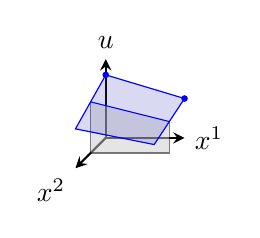
\begin{tikzpicture}
\draw[thick,-stealth] (0,0,0) coordinate(O) -- (1,0,0) node[right] {\(x^1\)};
\draw[thick,-stealth] (0,0,0) -- (0,1,0) node[above] {\(u\)};
\draw[thick,-stealth] (0,0,0) -- (0,0,1) node[below left] {\(x^2\)};
\coordinate (a) at (0,.8,0) {};
\coordinate (b) at (1,.5,0) {};
\coordinate (c) at (0,.5,1) {};
\coordinate (d) at (1,.3,1) {};
\coordinate (ac) at (0,.65,.5) {};
\coordinate (bd) at (1,.4,.5) {};
\draw[fill=black!20,opacity=.5] (ac) -- (0,0,.5) -- (1,0,.5) -- (bd);
\fill[blue] (a) circle (1.2pt);
\fill[blue] (b) circle (1.2pt);
\draw[blue,fill=blue!50!gray,opacity=.2] (a)--(c)--(d)--(b)--cycle;
\draw[blue] (a)--(c)--(d)--(b)--cycle;
\draw[blue] (ac)--(bd);
\end{tikzpicture}
\]
In other words, we need to see that these equations are compatible with one another.

\prob{test:CR.eqns}{Write out these differential equations for the exterior differential system of the Cauchy--Riemann equations in two complex variables.
Can you solve these differential equations, by specifying initial data as above?}
\prob{test:easy}{Prove that any involutive integral element of dimension \(p\), whose characters all vanish except perhaps \(s_{p-1}\) and \(s_p\), is tangent to an integral manifold.}
\prob{test:foliate}{Use the Cartan--K\"ahler theorem to prove that every involutive integral element of any exterior differential system lies tangent to a leaf of a foliation by integral manifolds, foliating some open set.
How many functions of how many variables do such foliations depend on?
Prove that any involutive integral manifold is covered in open sets, each of which is a leaf in a foliation by integral manifolds, foliating some open set.} 

\section{Compatibility and involutivity}
Geometrically, we sweep a point into an integral curve, sweep that into a surface, and so on.
Compatibility asks that the surface is an integral surface, and so on.
Suppose that the differential equations are compatible, i.e. we can pick any initial values in the domain of our coordinates, and obtain an integral manifold.
Then we can also pick initial values for the same differential equations nearby in those coordinates.
The space of integral elements, parameterized by the semipositive derivatives
\[
\pderiv{u^j}{x^{\legr{j}}},
\] 
has the predicted dimension at all nearby points.
So compatibility implies involutivity.

An incompatibility, arising as an additional differential equation, might vanish, perhaps to high order, at the particular point where we are working, but obstruct at nearby points. 
So we check the dimension of the space of integral elements nearby.

Incompatibilities can arise from commuting partial derivatives in our differential equations.
Any exterior differential system is closed under exterior derivative, expressing the commutativity of first partial derivatives.
So we expect that all incompatibilities are already present in the differential equations.
So we expect that incompatibilities force the dimension of nearby integral elements below the predicted dimension.
So we expect that compatibility is involutivity; chapter~\ref{chapter:proof} gives a proof.

\optionalSection{Generality of integral manifolds}%
As above, Cartan's strategy constructs integral manifolds of an involutive system by solving a sequence of determined equations, with initial data \(s_i\) functions of \(i\) variables, \(i=0,1,2,\dots,p\).
Count Taylor coefficients of initial data: the Taylor series of order \(k\) of integral manifolds, at a chosen point in our coordinates, form a manifold of dimension
\[
s_0+\binom{k}{0}s_1+\binom{k+1}{1}s_2+\dots+\binom{k+p-1}{p-1}s_p.
\]
As we vary \(k\), these dimensions of determine all of the characters.

Any other choice of determined systems of differential equations, giving rise to the same integral manifolds (or at least to the same Taylor series of integral manifolds at each order), injectively on each order of Taylor series, also has general solution depending on \(s_0\) constants, \(s_1\) functions of one variable, \(s_2\) functions of two variables, and so on.

\optionalSection{Deformation}%
A \emph{local deformation}\define{local deformation} of an integral manifold \(X\) is an analytic map \(\phi\) defined on an open subset of \(X\times\R\)  containing \(X\times\set{0}\) so that, for each constant \(t\), \(x\mapsto\phi(x,t)\) is an integral manifold, where defined, with \(\phi(x,0)=x\).
The \emph{velocity} of the deformation is the projection of
\(
\left.\pderiv{\phi}{t}\right|_{t=0}
\)
to the normal bundle of \(X\).
By deforming initial data, any integral manifold of any determined system is covered in open sets admitting local deformation with velocity any solution of the linearization.
We have not yet justified Cartan's strategy to prove the Cartan--K\"ahler theorem, but we can already see that, since the strategy is a sequence of determined problems, we can apply the same reasoning;
any involutive analytic integral manifold of any exterior differential system is covered in open sets admitting local deformation with velocity any solution of the linearization.
Local analytic velocity fields exist in the same generality as integral manifolds, solving linear determined problems.

The Holmgren uniqueness theorem \cite{John:1991} p. 80 proves that, on any analytic involutive integral manifold, any continuously differentiable velocity field is uniquely determined by its continuously differentiable initial data at each step in the sequence of linear determined problems.
However, existence of continuously differentiable velocity fields is not guaranteed.

\optionalSection{Prolongation}%
When we prolong, we form new equations \(\pi=p_j\omega^j\) for each polar.
Only the semipositive coefficients \(p^i_{\legr{i}}\) can vary freely. (For noninvolutive systems, not all of them vary freely.)
\[
d
\begin{pmatrix}
\pi^1-p^1_i\omega^1\\
\pi^2-p^2_i\omega^1\\
\vdots\\
\pi^p-p^p_i\omega^i
\end{pmatrix}
=
-
\begin{pmatrix}
dp^1_1 & *      & *      & \dots  & * \\
dp^2_1 & dp^2_2 & *      & \dots  & * \\
\vdots & \vdots & \vdots & \vdots & \vdots \\
dp^p_1 & dp^p_2 & \dots  & \dots  & dp^p_p
\end{pmatrix}
\wedge
\begin{pmatrix}
\omega^1 \\
\omega^2\\
\vdots\\
\omega^p
\end{pmatrix}
\]
modulo torsion, since we haven't included \(d\pi^i\) terms and \(d\omega^i\) terms.
The \(*\) terms are \(dp^i_j\) of negative grade, each solved for in terms of semipositive grade, so generate no polar.
There is no nonlinearity.
Some of these \(dp\) might be linearly dependent, due to noninvolutivity, so we don't know where to highlight polars, but the polars lie in some spots in among these semipositive \(dp\), on or below the diagonal.

Consider the characters \(s'_j\) of the prolongation.
There are \(s_1+s_2+\dots+s_p\) rows to this tableau, one for each polar, each representing a \(1\)-form in \(\II'\).
Grade zero in \(\II'\) also includes \(\II^1\), so
\[
s_0'=s_0+s_1+\dots+s_p.
\]
In the first column, there is at most one \(dp\) polar in each row:
\[
s_1'\le s_1+s_2+\dots+s_p.
\]
In the second column, 
\[
s_2'\le s_2+s_3+\dots+s_p,
\]
and so on, with finally \(s_p'\le s_p\): the last nonzero character cannot increase.
These inequalities are equalities just for involutive exterior differential systems.
